\documentclass{beamer}
\usetheme{Warsaw}
\useinnertheme{circles}
\useoutertheme[subsection=false]{smoothbars}
\usepackage[utf8x]{inputenc}
\usepackage[czech]{babel}
\usepackage[T1]{fontenc}
\usepackage{listings}
\usepackage{tikz}
\lstset{basicstyle=\tiny\ttfamily}
\logo{
\includegraphics[height=0.5cm]{brmlab.pdf}}

\begin{document}

\AtBeginSection[]
{
  \begin{frame}
    \frametitle{Outline}
    \tableofcontents[currentsection]
  \end{frame}
}

\title{brmiversity: Umělá inteligence\\a teoretická informatika}
\subtitle{Přednáška č. 3}
\author{Petr Baudiš $\langle${\tt pasky@ucw.cz}$\rangle$}
\institute{
	brmlab 2011\\
	\vskip 1ex
	\pgfdeclareimage[height=4ex]{ccbysa}{by-sa.pdf}
	\pgfuseimage{ccbysa}
}
\date{}
\frame{\titlepage}

\section{Adaptivní agenti}

\subsection{}
\begin{frame}{Autonomní adaptivní agent (umělá bytost)}
(Velmi inspirováno slajdy Cyrila Broma.)
\begin{itemize}
\item Virtuální bytost, ve virtuálním nebo skutečném prostředí, autonomní, s vlastním tělem
\vskip 3ex
\item Artificial mind is a piece of code that decides ``what to do next''
\item The problem of deciding what to do next is called the action selection problem
\item To decide what to do next, the creature must perceive its environment
\item An action causes a change in the environment, and it usually has a feedback on the creature
\end{itemize}
\end{frame}

\subsection{}
\begin{frame}{Architektura agenta}
\begin{columns}
\begin{column}{5cm}
Non-free artwork,
viz slajdy Cyrila Broma k Umělým bytostem.
%\includegraphics[width=5cm]{arch1.png} \\
%\includegraphics[width=5cm]{arch2.png}
\end{column}
\begin{column}{7cm}
\begin{itemize}
\item Reaktivní ``plánování'': ``Turingův stroj'' --- na základě stavu a podnětu akce + nový stav; vlastně se neplánuje
\item If-then pravidla: Když se stane X, udělej Y, sada uspořádaných pravidel s prioritou
\item Konečný automat: viz minule
\item Neuronové sítě atd.
\end{itemize}
\end{column}
\end{columns}
\end{frame}

\subsection{}
\begin{frame}{Architektura agenta}
\begin{itemize}
\item POSH: Parallel-rooted, Ordered Slip-stack Hierarchical: Hierarchická if-then pravidla; akce, kompetence, ``pudy''
\item Belief Desire Intention: Možná špatné beliefs, množina desires, některé z nich vybrané jako intentions
\item Soar: State, Operator And Result (Input; Proposing -- Decision -- Applying; Output)
\end{itemize}
\end{frame}

\subsection{}
\begin{frame}{Otázky?}
\begin{center}
Příště: Pohyb agentů --- navigace v prostoru.
\end{center}
\end{frame}

\section{Evoluční algoritmy}

\subsection{}
\begin{frame}{Umělá evoluce}
\begin{itemize}
\item Příroda: Živí jedinci jsou (částečně) popsáni svojí DNA, ta se mění s časem podle působení přírodního výběru
\item Programy: Jedinci odpovídající problémům jsou popsáni nějak kódovaným řetězcem, ten se mění s časem podle působení výběru (selekce) na základě fitness
\item Kódování: Řetězec hodnot
\item Fitness: Ohodnocení výkonu jedince
\item Změna jedince: Operace na kódování --- mutace a křížení
\item Velká populace mnoha jedinců!
\end{itemize}
\end{frame}

\subsection{}
\begin{frame}{Genetické operátory}
\begin{itemize}
\item {\bf Selekce} --- ohodnotíme množinu jedinců WTF
\item {\bf Mutace} --- $\forall i$ s (velmi nízkou) pravděpodobností $p$ změníme hodnotu prvku $i$ jedince
\item {\bf Křížení} --- vyrobíme nového jedince rekombinací řetězců dvou jedinců
\end{itemize}
\end{frame}

\subsection{}
\begin{frame}{Genetický algoritmus}
\begin{itemize}
\item Máme populaci předchozí generace, vyrábíme novou generaci (dokud nenajdeme optimum).
\item Nová generace (dokud není plná):
\begin{itemize}
\item Vyber dva jedince z minulé populace (selekce)
\item Vyrob dva nové jedince (křížení)
\item Zmutuj jedince
\item Dvojici vlož do nové generace
\end{itemize}
\item Elitismus a spoustu dalších vylepšení
\end{itemize}
\end{frame}

\subsection{}
\begin{frame}{Otázky?}
\begin{center}
Příště: Reprezentační schémata, evoluční a genetické programování.
\end{center}
\end{frame}

\section{Základní algoritmy}

\subsection{}
\begin{frame}{Minimální kostra grafu}
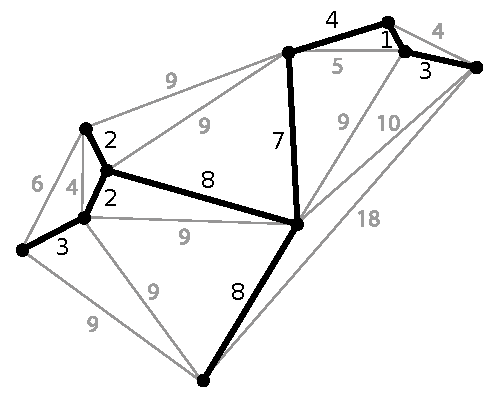
\includegraphics[width=9cm]{Minimum_spanning_tree.pdf}
\end{frame}

\section{Datové struktury}

\subsection{}
\begin{frame}{Halda}
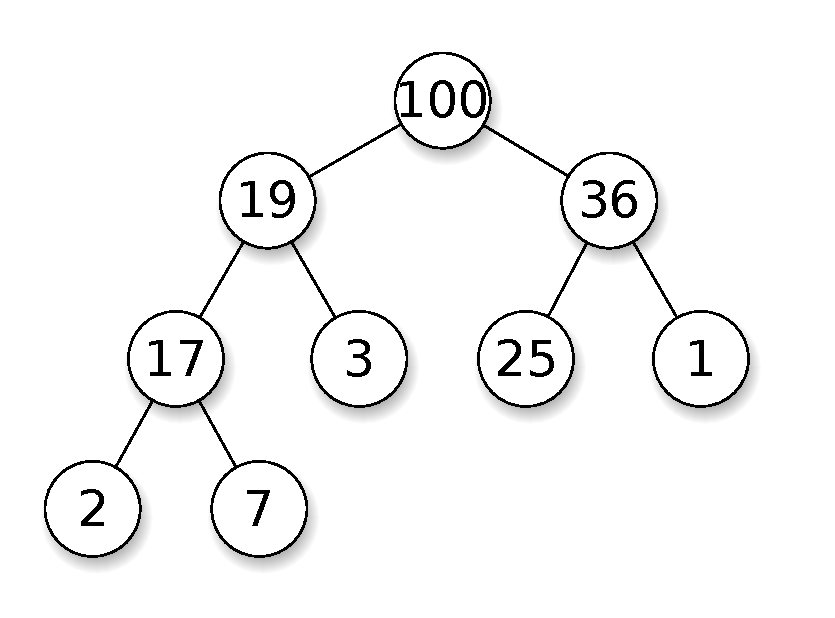
\includegraphics[width=4cm]{Heap.pdf}
\begin{itemize}
\item Chceme ukládat data tak, abychom vždy mohli snadno vytáhnout minimum
\item Prioritní fronta, např. na minimální kostru grafu :-)
\pause
\item \dots cože?
\pause
\item Speciálně uspořádaný strom: synové jsou vždy větší než otec
\item Tedy v kořeni je nejmenší prvek
\item Zejména operace INSERT, DELETEMIN
\end{itemize}
\end{frame}

\subsection{}
\begin{frame}{Regulární halda}
\begin{itemize}
\item Pěkně ``zarovnaný'' strom, každý otec \\ kromě těch u dna má dva syny \\ (má hloubku $\log n$)
\item Mezi syny není žádné pořadí
\item INSERT: Přidáme na ``konec'' haldy \\ (na dně), posouváme nahoru, dokud je porušena podmínka
\item DELETEMIN: Prohodíme kořen a poslední prvek, umažeme poslední prvek, prvek z kořene posouváme dolů
\item Složitosti $O(\log n)$
\item Heap sort!
\end{itemize}
\begin{tikzpicture}[remember picture,overlay]
  \node [xshift=-4.5cm,yshift=-5cm,above right] at (current page.north east)
    {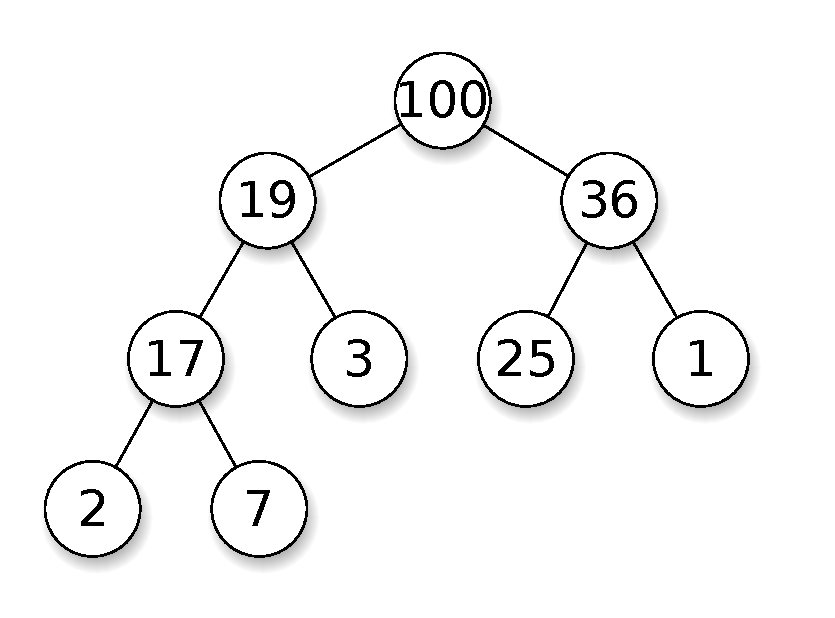
\includegraphics[width=4cm]{Heap.pdf}};
\end{tikzpicture}
\end{frame}

\subsection{}
\begin{frame}{Levicové (leftist) haldy}
\begin{itemize}
\item Místo probublávání budeme mít jako základní operaci MERGE dvou hald.
\item Línější strukturální podmínka; levý syn má vždy delší cestu k nejbližšímu listu.
\item MERGE prohazuje uzly podle uspořádání, syny podle cesty k listu, rekurze do {\em pravého} syna.
\end{itemize}
\end{frame}

% \subsection{}
% \begin{frame}{Binomiální haldy}
% \begin{itemize}
% \item TODO
% \end{itemize}
% \end{frame}
% 
% \subsection{}
% \begin{frame}{Fibonacciho haldy}
% \begin{itemize}
% \item TODO
% \end{itemize}
% \end{frame}

\subsection{}
\begin{frame}{Otázky?}
\begin{center}
Příště: Složitější haldy. Hashovací algoritmy.
\end{center}
\end{frame}

\section{Složitost}

\subsection{}
\begin{frame}{Rekapitulace: P a NP}
\begin{itemize}
\item P: Třída problémů řešitelných v polynomiálním čase $O(n^k)$ na DTS (Turingově stroji)
\item NP: Třída problémů řešitelných v polynomiálním čase $O(n^k)$ na NTS (nedeterministickém Turingově stroji)
\item NTS: Nepřecházíme do jednoznačného dalšího stavu programu, ale do několika možných
\item (V praxi musíme NTS simulovat na DTS a vykonávat postupně všechny možné větve výpočtu --- exponenciální časová složitost $O(2^n)$)
\item (Konsekvence NP: {\em Certifikát} NP problému (popis větvení programu) lze ověřit v polynomiálním čase na DTS.)
\item Může být nějaký program ještě pomalejší než NP?
\pause
\item Může! EXPTIME (Go)
\end{itemize}
\end{frame}

\subsection{}
\begin{frame}{Úplné problémy}
\begin{itemize}
\item Problém je ve třídě NP: Dá se v polynomiálním čase spočítat na NTS. \\ {\em (Popíšeme, jak certifikát ověřit v p. čase.)} \\ V NP jsou i všechny {\em lehčí} problémy!
\item Problém je NP-těžký: Každý problém z NP lze \only<2,3>{v polynomiálním čase} převést na ten náš \\ {\em (Napíšeme program, který to dělá.)}
\item Problém je NP-úplný: Problém je NP a NP-těžký
\pause
\pause
\item Je to zábava, lépe pochopíme vlastnosti třídy NP
\item P=NP dokážeme na jednom NP-úplném algoritmu, můžeme pak v P řešit všechny
\item Některé NP problémy umíme heuristicky rychle řešit ``skoro dokonale'' (3SAT), aplikujeme na jiné problémy
\end{itemize}
\end{frame}

\subsection{}
\begin{frame}{Kachlíkování}
\begin{columns}
\begin{column}{6cm}
\begin{itemize}
\item Máme sadu barev a sadu kachlíků s různě obarevnými hranami. K sobě patří kachlíky se stejně barevnými hranami
\item Obdélníkové pole (``koupelna''), vstupní hrana s obarvenými ``bity'', výstupní hrana, kterou musíme obarvit
\item Program jsou barvy a kachlíky!
\vskip 3ex
\item Texturování v počítačové grafice
\item Proteiny místo kachliček --- biologické výpočty
\end{itemize}
\end{column}
\begin{column}{5cm}
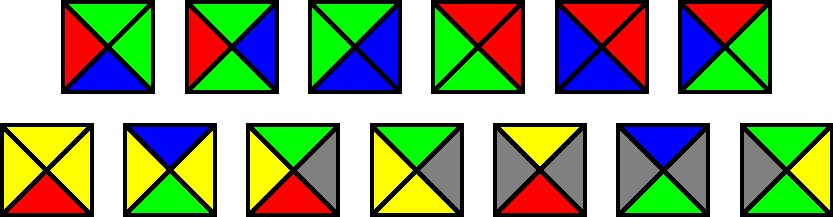
\includegraphics[width=5cm]{Wang_tiles.pdf} \\
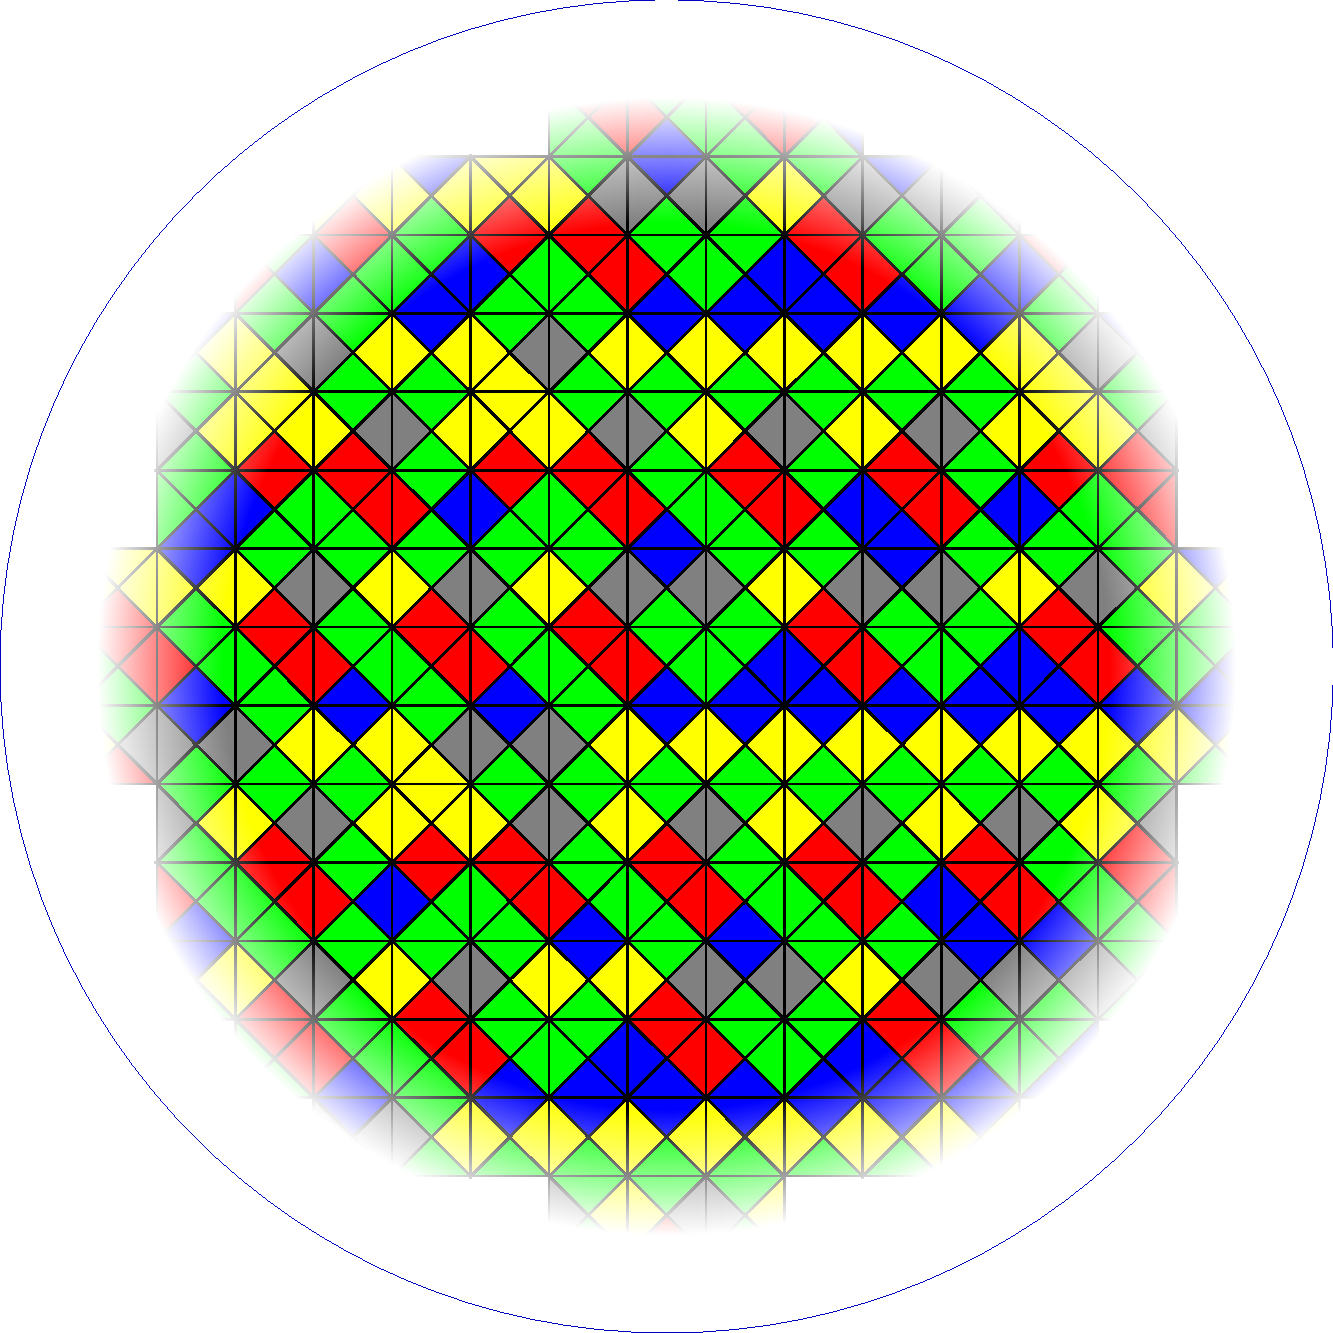
\includegraphics[width=5cm]{Wang_tesselation.pdf} \\
\end{column}
\end{columns}
\end{frame}

\subsection{}
\begin{frame}{TS na kachlíkování}
\begin{itemize}
\item Intuice: Najít vykachlíkování je těžké (Eternity). Ověřit předložené vykachlíkování (postup běhu programu, certifikát) je snadné.
\item Problém je v NP (řešení ověříme rychle)
\vskip 3ex
\item Jak dokázat, že je problém NP-těžký?
\pause
\item (i) Převedeme na něj jiný NP-těžký \\ (ii) Budeme s ním simulovat Turingův stroj
\end{itemize}
\end{frame}

\subsection{}
\begin{frame}{TS na kachlíkování}
\begin{itemize}
\item Kachlíkujeme po řádcích, první řádek (vstupní hrana) je vstupní páska
\item V každém řádku bude zakódovaný jeden krok Turingova stroje
\item Hrany od vstupní k výstupní hraně: stav pásky před krokem, za krokem \\ highlight buňky pod hlavou \\ hrany mezi buňkami řádku: přechody hlavy
\end{itemize}
Non-free artwork, viz skripta Vladana Majerecha ``Úvod do složitosti a NP-úplnosti''.
%\includegraphics[width=10cm]{kachl-ts.png}
\end{frame}

\subsection{}
\begin{frame}{SAT}
\begin{itemize}
\item Satisfiability: Vstup je logický výraz v ``konjunktivní normální formě'':
$$ (a \lor b \lor \neg c) \land (\neg \lor a \lor b \lor \neg c) $$
Existuje splňující kombinace logických hodneg proměnných?
\item Dá se převést kachlíkování na 3-SAT
\item $x_{i,j,k}$ kachlíček $k$ na souřadnicích $i,j$
\item $\neg x_{i,j,k} \lor \neg x_{i,j,k'}$, $x_{i,j,k} \lor x_{i,j,k'}$
\item $\neg x_{i,j,k} \lor \neg x_{i,j+1,k'}$ a analogicky pro $i$ podle barev
\end{itemize}
\end{frame}

\subsection{}
\begin{frame}{3-SAT}
3-Satisfiability: trojliterálové závorky
$$ (a \lor b \lor \neg c) \land (\neg \lor a \lor b \lor \neg c) $$

SAT: Obecný počet literálů. Převedeme ho na 3-SAT, pro delší závorky vyrobíme pomocné literály:
$$ (a \lor \neg b \lor c \lor d) $$
$$ (a \lor \neg b \lor x_1) \land (\neg x_1 \lor c \lor x_2) \land (\neg x_2 \lor d \lor 1) $$
\end{frame}

\subsection{}
\begin{frame}{Hamiltonovská kružnice}
\begin{columns}
\begin{column}{2cm}
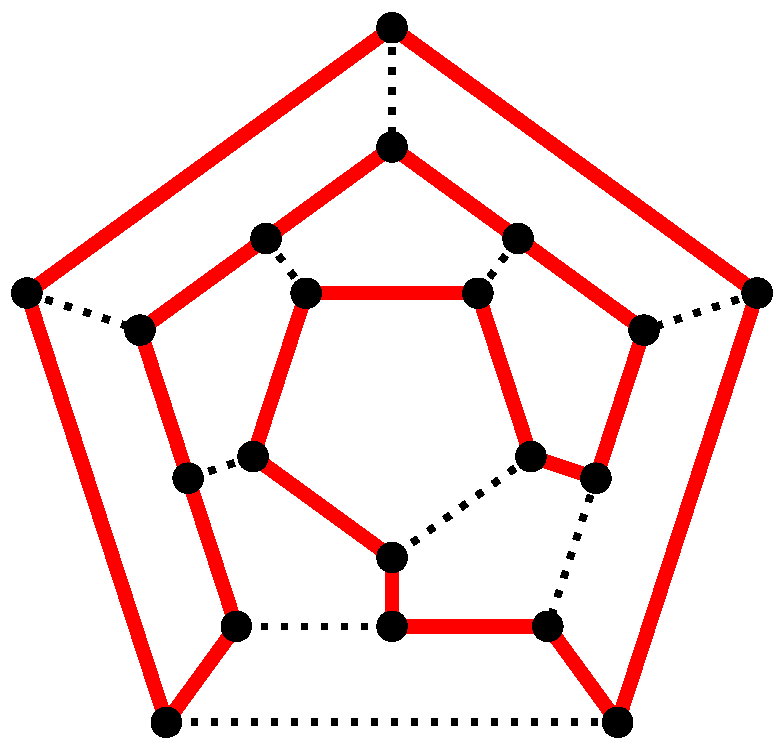
\includegraphics[width=2cm]{Hamiltonian_path.pdf} \\
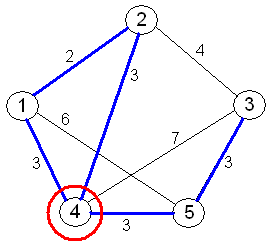
\includegraphics[width=2cm]{TSP.png}
\end{column}
\begin{column}{10cm}
\begin{itemize}
\item Chceme navštívit všechny vrcholy grafu, abychom každý navštívili právě jednou.
\item SAT umíme převést na HK
\end{itemize}
\end{column}
\end{columns}
Non-free artwork, viz skripta Vladana Majerecha ``Úvod do složitosti a NP-úplnosti''.
%\includegraphics[width=8cm]{hk-sat.png}
\end{frame}

\subsection{}
\begin{frame}{Otázky?}
\begin{center}
Příště: Metody tvorby algoritmů. (Problém batohu později.)
\end{center}
\end{frame}

\subsection{}
\begin{frame}{Děkuji vám}
\begin{center}
{\bf pasky@ucw.cz}

Příště: Neuronové sítě, umělá inteligence (hry), \\ složitost, vyčíslitelnost (halting problem).
\end{center}
\end{frame}

\end{document}
